\section{Methods}\label{methods}
The methods for implementation of a behavioral, discrete-time PLL simulator and for the PLL loop filter automation and optimization will be covered here.

\hl{Talk about how simulator is implemented:}
\hl{Discrete simulation models of phase noise, dco etc}
\hl{Filter optimization}
\hl{-phase noise and lock time estimate in frequency domain}

\subsection{Behavioral, discrete event PLL simulation}
To fully capture the effects of a discrete time PLL with digital quantization effects, the implementation a behavioral, discrete event PLL simulator is described in the following. The simulator utilizes of behavioral models of to describe the individual components which comprise the PLL. These components are (1) a clock reference, (2) a TDC, (3) a loop filter, (4) a DCO, and (5) a divider. These behavioral models fully encapsulate effects of time-quantization and digitization. The simulator operates by iterating in fixed time steps of $\Delta t$, where each node in the PLL is updated based upon the previous node values in a manner that is defined by each PLL component behavioral model. Each behavioral model is represented programmatically utilizing classes. In simulation, each component instance is represented by a object instance of the respective model class, constructed with any initial parameters (such as division ratio) that describe the component.
\begin{figure}[htb!]
	\center\fontfamily{\sfdefault}\selectfont
% XCircuit output "simulator.tex" for LaTeX input from simulator.ps
\def\putbox#1#2#3#4{\makebox[0.00000in][l]{\makebox[#1][l]{}\raisebox{\baselineskip}[0.00000in][0.00000in]{\raisebox{#2}[0.00000in][0.00000in]{\scalebox{#3}{#4}}}}}
\def\rightbox#1{\makebox[0.00000in][r]{#1}}
\def\centbox#1{\makebox[0.00000in]{#1}}
\def\topbox#1{\raisebox{-0.60\baselineskip}[0.00000in][0.00000in]{#1}}
\def\midbox#1{\raisebox{-0.20\baselineskip}[0.00000in][0.00000in]{#1}}
   \scalebox{1}{
   \normalsize
   \parbox{6.30936in}{
   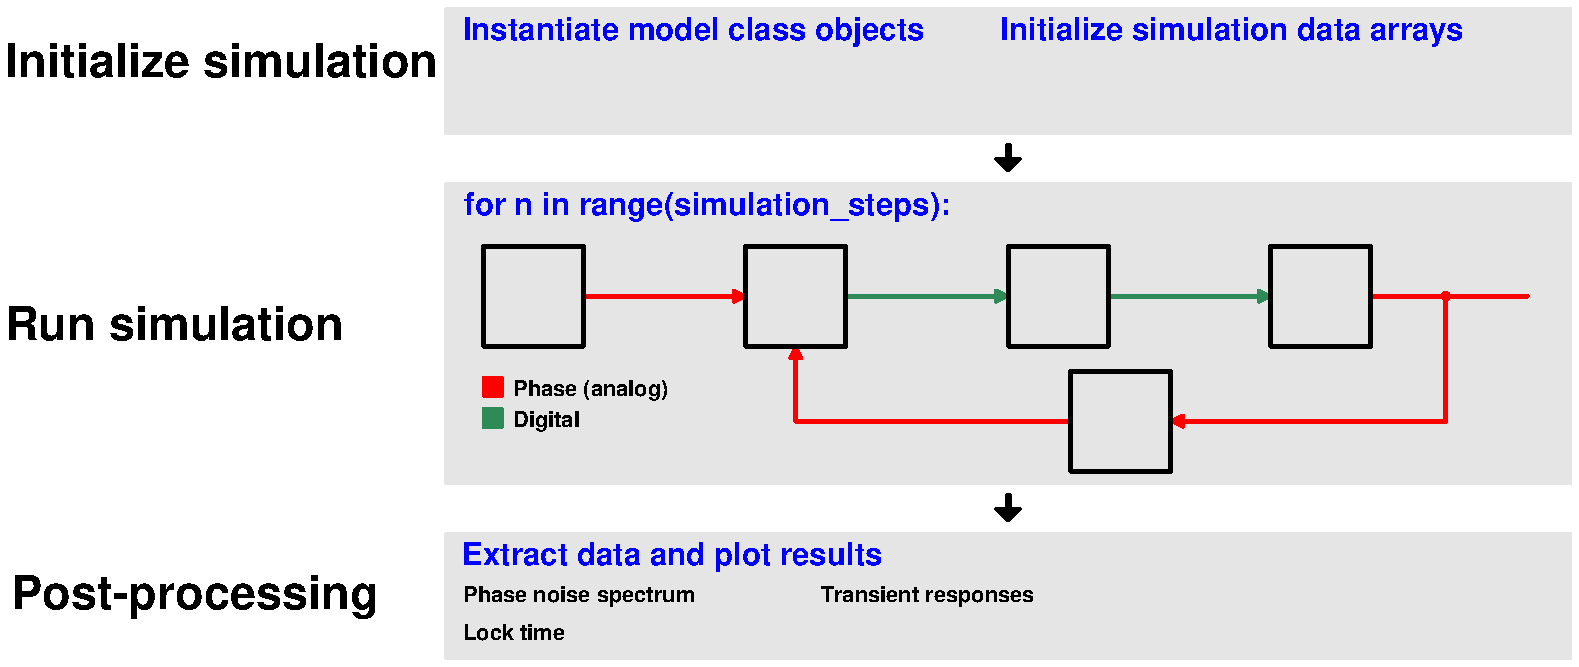
\includegraphics[scale=0.60000]{./figs/simulator.pdf}\\
   % translate x=1040 y=384 scale 0.38
   \putbox{3.08400in}{1.45800in}{0.84}{\texttt{tdc}}%
   \putbox{4.38600in}{0.96000in}{0.84}{\texttt{div}}%
   \putbox{4.17000in}{1.45800in}{0.84}{\texttt{lf}}%
   \putbox{5.18400in}{1.45800in}{0.84}{\texttt{dco}}%
   \putbox{2.03400in}{1.45800in}{0.84}{\texttt{clk}}%
   \putbox{3.48600in}{1.03200in}{0.84}{\texttt{div\_sig[n]}}%
   \putbox{2.38200in}{1.56000in}{0.84}{\texttt{clk\_sig[n]}}%
   \putbox{3.43200in}{1.54800in}{0.84}{\texttt{tdc\_sig[n]}}%
   \putbox{4.48200in}{1.54800in}{0.84}{\texttt{lf\_sig[n]}}%
   \putbox{5.53200in}{1.54800in}{0.84}{\texttt{dco\_sig[n]}}%
   \putbox{4.00800in}{2.35800in}{0.84}{\texttt{clk\_sig[n]}}%
   \putbox{4.00800in}{2.20800in}{0.84}{\texttt{tdc\_sig[n]}}%
   \putbox{4.71000in}{2.35800in}{0.84}{\texttt{lf\_sig[n]}}%
   \putbox{4.71000in}{2.20800in}{0.84}{\texttt{dco\_sig[n]}}%
   \putbox{5.38200in}{2.35800in}{0.84}{\texttt{div\_sig[n]}}%
   \putbox{1.86000in}{2.35800in}{0.84}{\texttt{clk}}%
   \putbox{1.86000in}{2.20800in}{0.84}{\texttt{tdc}}%
   \putbox{2.40600in}{2.35800in}{0.84}{\texttt{lf}}%
   \putbox{2.40600in}{2.20800in}{0.84}{\texttt{dco}}%
   \putbox{2.95800in}{2.35800in}{0.84}{\texttt{div}}%
   \putbox{1.88400in}{0.83400in}{0.84}{t$_{sim}$ = \texttt{n}$\Delta$t}%
   \putbox{2.73600in}{3.09600in}{0.72}{\texttt{fref}}%
   \putbox{2.55600in}{2.99400in}{0.72}{\texttt{div\_n}}%
   \putbox{2.49600in}{2.89800in}{0.72}{\texttt{tdc\_steps}}%
   \putbox{3.60600in}{3.09600in}{0.72}{\texttt{kdco}}%
   \putbox{4.20600in}{2.99400in}{0.72}{\texttt{dco\_f0}}%
   \putbox{4.20600in}{2.89800in}{0.72}{\texttt{dco\_pn}}%
   \putbox{5.64600in}{3.09600in}{0.72}{\texttt{init\_f\_error}}%
   \putbox{5.18400in}{2.99400in}{0.72}{\texttt{lf\_params}}%
   \putbox{5.44800in}{2.89800in}{0.72}{\texttt{sim\_steps}}%
   } % close 'parbox'
   } % close 'scalebox'
   \vspace{-\baselineskip} % this is not necessary, but looks better
\fontfamily{\rmdefault}\selectfont

	\caption{Simulation process.}
	\label{fig:simulator}
\end{figure}
\FloatBarrier
The discrete event simulator is given in the following pseudocode, with component model objects \{\texttt{clk, tdc, lf, dco, div}\}, and simulation data arrays \{\texttt{clk\_sig, tdc\_sig, lf\_sig, dco\_sig, div\_sig}\}. Each model object is updated at each simulation step utilizing the class method \texttt{update}, passing any relevant simulation data as arguments to the method.

\begin{lstlisting}[language={Python}, caption={PLL simulation loop Python pseudocode}, label={sim_code}]
for n in range(simulation_steps):
    clk_sig[n] = clk.update()
    tdc_sig[n] = tdc.update(clk_sig[n-1], div_sig[n-1]))
    lf_sig[n]  = lf.update(tdc_sig[n-1], clk_sig[n-1]) #loop filter
    osc_sig[n] = dco.update(lf_sig[n-1])
    div_sig[n] = div.update(osc_sig[n-1], div_n)
    \end{lstlisting}
After the simulation loop reaches completion, the results stored in the simulation data arrays can be post-processed to extract phase noise data, transient behavior and lock time. The following sections will discuss in more detail the implemented behavioral model classes and post-processing.

\subsubsection{Clock behavioral model}
An ideal behavioral clock model is utilized. The model is instantiated with the clock frequency \texttt{f} and the simulator time step \texttt{dt}. The model functions by incrementing its phase every simulation step by $\Delta \Phi$ = $2\pi$\texttt{f}$\cdot$\texttt{dt}. The model outputs an analog phase signal.

\begin{lstlisting}[language={Python}, caption={Ideal clock behavioral model.}, label={clk_code}]
class Clock:
	def __init__(self, f, dt):
		self.f = f 			# clock frequency
		self.dt = dt 		# simulation time step
		self.phase = 0.0	# clock phase state variable

	def update(self):
		self.phase += 2*pi*self.f*self.dt 	# increment phase
		return self.phase
    \end{lstlisting}

\subsubsection{TDC behavioral model}
The TDC behavioral model takes two analog inputs \texttt{x} and \texttt{y} that are in units of phase, and outputs a digital word that quantifies the phase separation of the signals. The model is instantiated with a resolution parameter \texttt{tdc\_steps}, which defines the number of phase steps per cycle of the reference input \texttt{x} the TDC can resolve.

\begin{lstlisting}[language={Python}, caption={TDC behavioral model.}, label={tdc_code}]
class TDC:
	def __init__(self, tdc_steps):
		self.tdc_steps = tdc_steps

	def update(x, y):
		ph_error = wrap(x-y) 	# wraps phase to be within [0, 2*pi]
		return round(self.tdc_steps*(ph_error/(2*pi)))
\end{lstlisting}
\subsubsection{Loop filter behavioral model}
The loop filter model implements a discrete-time filter via difference equation that operates on input \texttt{x}. The equivalent of one pole and two zeros are modelled, described using the filter coefficients $\{a_1, a_2; b_0, b_1\}$:
\begin{equation}
\text{H}_{LF}(z) = \frac{b_0 + b_1z^{-1}}{a_0 + a_1z^{-1} + a_2z^{-2}}
\end{equation}
\begin{equation}
\text{y}[n] = -a_1 \text{y}[n-1]-a_2 \text{y}[n-2] + b_0\text{x}[n] + b_1\text{x}[n-1]
\end{equation}
Pseudocode for implementation of the model class is as follows. Data is to be represented with fixed point format, with number of fractional bits \texttt{frac\_bits} and number of integer bits \texttt{int\_bits}. A method \texttt{fixed\_point} is used to round floating point values to be equivalent to the nearest representation in the desired fixed point format given with (int\_bits.frac\_bits)$_2$. The filter coefficients are assumed to be pre-converted to the desired fixed-point equivalent values, and input \texttt{x} is assumed to be integer-valued.
\begin{lstlisting}[language={Python}, caption={Loop filter behavioral model.}, label={lf_code}]
class LoopFilter:
	def __init__(self, a1, a2, b0, b1, int_bits, frac_bits):
		self.a1 = a1;	self.a2 = a2
		self.b0 = b0;	self.b1 = b1
		self.xprev1 = 0;	
		self.yprev1 = 0; self.yprev2 = 0
		self.int_bits=int_bits;	self.frac_bits=frac_bits

	def update(x):
		ynew = -self.a1*self.yprev1 - self.a2*self.yprev2 \\
			   + self.b0*x + self.b1*self.xprev1	# difference equation
		self.yprev2 = self.yprev1	
		self.yprev1 = fixed_point(ynew, self.int_bits, self.frac_bits)
		self.xprev1 = x
		return round(self.yprev1)	# convert to integer
\end{lstlisting}

\subsubsection{DCO behavioral model}
The DCO is modeled similar to the clock, except with a digital input \texttt{otw} for tuning the frequency. Additionally, oscillator phase noise modeling is included utilizing a random phase walk component \hl{cite theory}. Random walk is implemented by stochastically adding $\pm$\texttt{krw} in phase to the oscillator phase every
simulation step. The sign of the added amount \texttt{krw} is randomly chosen with equal probability for positive and negative, implemented with via method \texttt{choice}. 
\begin{lstlisting}[language={Python}, caption={DCO behavioral model.}, label={dco_code}]
class DCO:
	def __init__(self, f0, kdco, krw):
		self.f0 = f0		# nominal frequency
		self.kdco = kdco 	# DCO gain
		self.krw			# random phase walk gain
		self.phase = 0		# phase state variable

	def update(otw):
		self.phase += 2*pi*(f0 + otw*kdco) + krw*choice([-1,1])
		return self.phase
    \end{lstlisting}

\subsubsection{Divider behavioral model}
The divider model is definied with the divider modulus \texttt{div\_n} and
\begin{lstlisting}[language={Python}, caption={Divider behavioral model.}, label={div_code}]
class Divider:
	def update(x, div_n):
		return x/div_n
\end{lstlisting}
\subsubsection{Post-processing}

\subsubsection{Monte-Carlo sampling}
An engine for automated simulation of parameter variations...
	\hl{Used to verify stability}

\subsection{Loop filter optimization}
	Reference phase noise does not matter, is always fixed.
	DCO and TDC phase noise should be highest. Will simulate with other noise sources, but framework will optimize loop filter design and provide recommendations for other parameters (max divider jitter) so DCO and TDC phase noise are dominant.
\subsubsection{Estimation of settling time}

	Based on a continuous model of the PLL dynamics, the PLL closed loop phase transfer function $\mathrm{T}(s)$ is defined in the following form, where number of poles P $>$ number of zeros Z. The transfer function is defined as a rational function of two polynomial functions of s. 
	\begin{equation}\label{eq:pll_cl_tf}
	\mathrm{T}(s) = \frac{\sum_{j=0}^Z b_js^j}{\sum_{k=0}^P a_ns^n}
	\end{equation}
	An estimate of the step response settling time of $\mathrm{T}(s)$ can by utilizing its representation in state space. This is given in \ref{eq:ss_rep}, with input vector $\mathrm{U}(s)$, state vector $\mathbf{X}(s)$,  and output $\mathbf{Y}(s)$. The state-space representation from a s-domain transfer function can be quickly solved computationally with available signal processing packages such as \texttt{scipy.signal}.
	% https://lpsa.swarthmore.edu/Representations/SysRepTransformations/TF2SS.html
	\begin{align} \label{eq:ss_rep}
		s\mathbf{X}(s) &= \mathbf{AX}(s) +\mathbf{B}\mathrm{U}(s)\\
		Y(s) &= \mathbf{CX}(s) +\mathbf{D}\mathrm{U}(s)
	\end{align}
	The set of k eigenvalues $\{\lambda_1, ... , \lambda_{N}\}$ corresponding to poles for the system are found as the roots of \ref{eq:ss_eigenvals}.% The associated eigenvectors are found with \ref{eq:ss_eigenvecs}.
	\begin{align}
		|\mathbf{A} - \lambda \mathbf{I}| = 0\label{eq:ss_eigenvals}%\\
		%\mathbf{A} \mathbf{v}_k = \lambda_k\mathbf{v}_k \label{eq:ss_eigenvecs}
	\end{align}
	With the constraint of number of poles $>$ number of zeros, the system $\mathrm{T}(s)$ may be represented via partial fraction decomposition using the poles from the eigenvalues of state matrix $\mathbf{A}$ $\{\lambda_1, ... , \lambda_{N}\}$:
	\begin{equation}
		T(s) = \sum_{k=1}^{P} \frac{c_k}{s-\lambda_k}
	\end{equation}
	The step response of this system will take the form as a sum of complex exponentials:
	\begin{equation}
		y(t) = c_1e^{\lambda_1t} + ... + c_ke^{\lambda_kt}%, \hspace{1em} \mathbf{y(t)} = [ y(t) \hspace{0.5em}y^{'}(t)\hspace{0.5em} ...\hspace{0.5em} y^{(k)}(t)]^T
	\end{equation}

	% The state transition matrix $\mathbf{\Phi}_{\mathrm{T}}$ corresponding to the system $\mathrm{T}(s)$ is:
	% \begin{equation}
		% \mathbf{\Phi}_\mathrm{T} = (s\mathbf{I}-A)^{-1}
	% \end{equation}

	The dynamics of the step response are governed by the exponential components of y(t). If  $\{\lambda_1, ... , \lambda_N\} \in \mathds{C}$ where $\lambda_k=\sigma_k+j\omega_K$, the real portion of each $\lambda_k$ will describe the transient behavior. The long term settling of y(t) will be dominated by the $\lambda_k$ with the smallest valued real component, that is the dominant pole. This value is approximately the reciprocal time constant for the system. Settling time $t_s$ can be considered as the interval required for the signal to drop within a tolerance band $\pm \delta_{tol} \textnormal{y}(\infty)$ about the final value $\textnormal{y}(\infty)$. 
	\begin{equation}
		t_s = \tau\ln(\delta_{tol}) = \frac{\ln(\delta_{tol})}{\min(|\Re(\{\lambda_1, ... , \lambda_k\})|)}
	\end{equation}
	This settling time estimate is computationally fast, as it requires only (a) computation of state matrix $\mathbf{A}$, (b) computation of the eigenvalues of $\mathbf{A}$, and (c) computation of settling time from the eigenvalue with minimum real component.
\subsubsection{Estimation of PLL phase noise}
	It is assumed that the dominant output-referred phase noise contributions are due to the DCO thermal noise and the TDC quantization. If such is the case, total output integrated noise power is at a minimimum when the TDC and DCO contributions are approximately equal. Thus $S_{TDC}$ and $S_{DCO}$ are the PLL output-referred noise PSD respectively for the TDC and DCO noise sources. The total PLL output noise PSD $S_{\Sigma}(f)$ is (N is the PLL divider modulus):
	\begin{equation}
		S_{\Sigma}(f) = f_{clk}\cdot|2\pi N\cdot G(f)|^2S_{TDC} + |1-G(f)|^2S_{DCO}
	\end{equation}

	Given a bandwidth of interest $\Delta f$ (i.e. baseband bandwidth for radio applications), the total integrated phase noise power is:
	\begin{equation}
		P_{\phi noise} = 2\int_0^{\Delta f} S_{\Sigma}(f)df
	\end{equation}
	This can be computation solved for a grid of K values in the interval $\Delta f$, where each point represents a frequency bin $f_{bin}$ = $\Delta f$/K. Therefore this estimate is implemented as such:
	\begin{equation}
		\hat{P}_{\phi noise} = 2\sum_{k=0}^{K-1} S_{\Sigma}(kf_{bin})f_{bin}
	\end{equation}

\subsubsection{Optimization algorithm}
	Utilize BFGS optimization with constraints on settling time
